\chapter{Схема принципиальная электрическая}
\label{pril:A}
\begin{figure}[h!]
\center{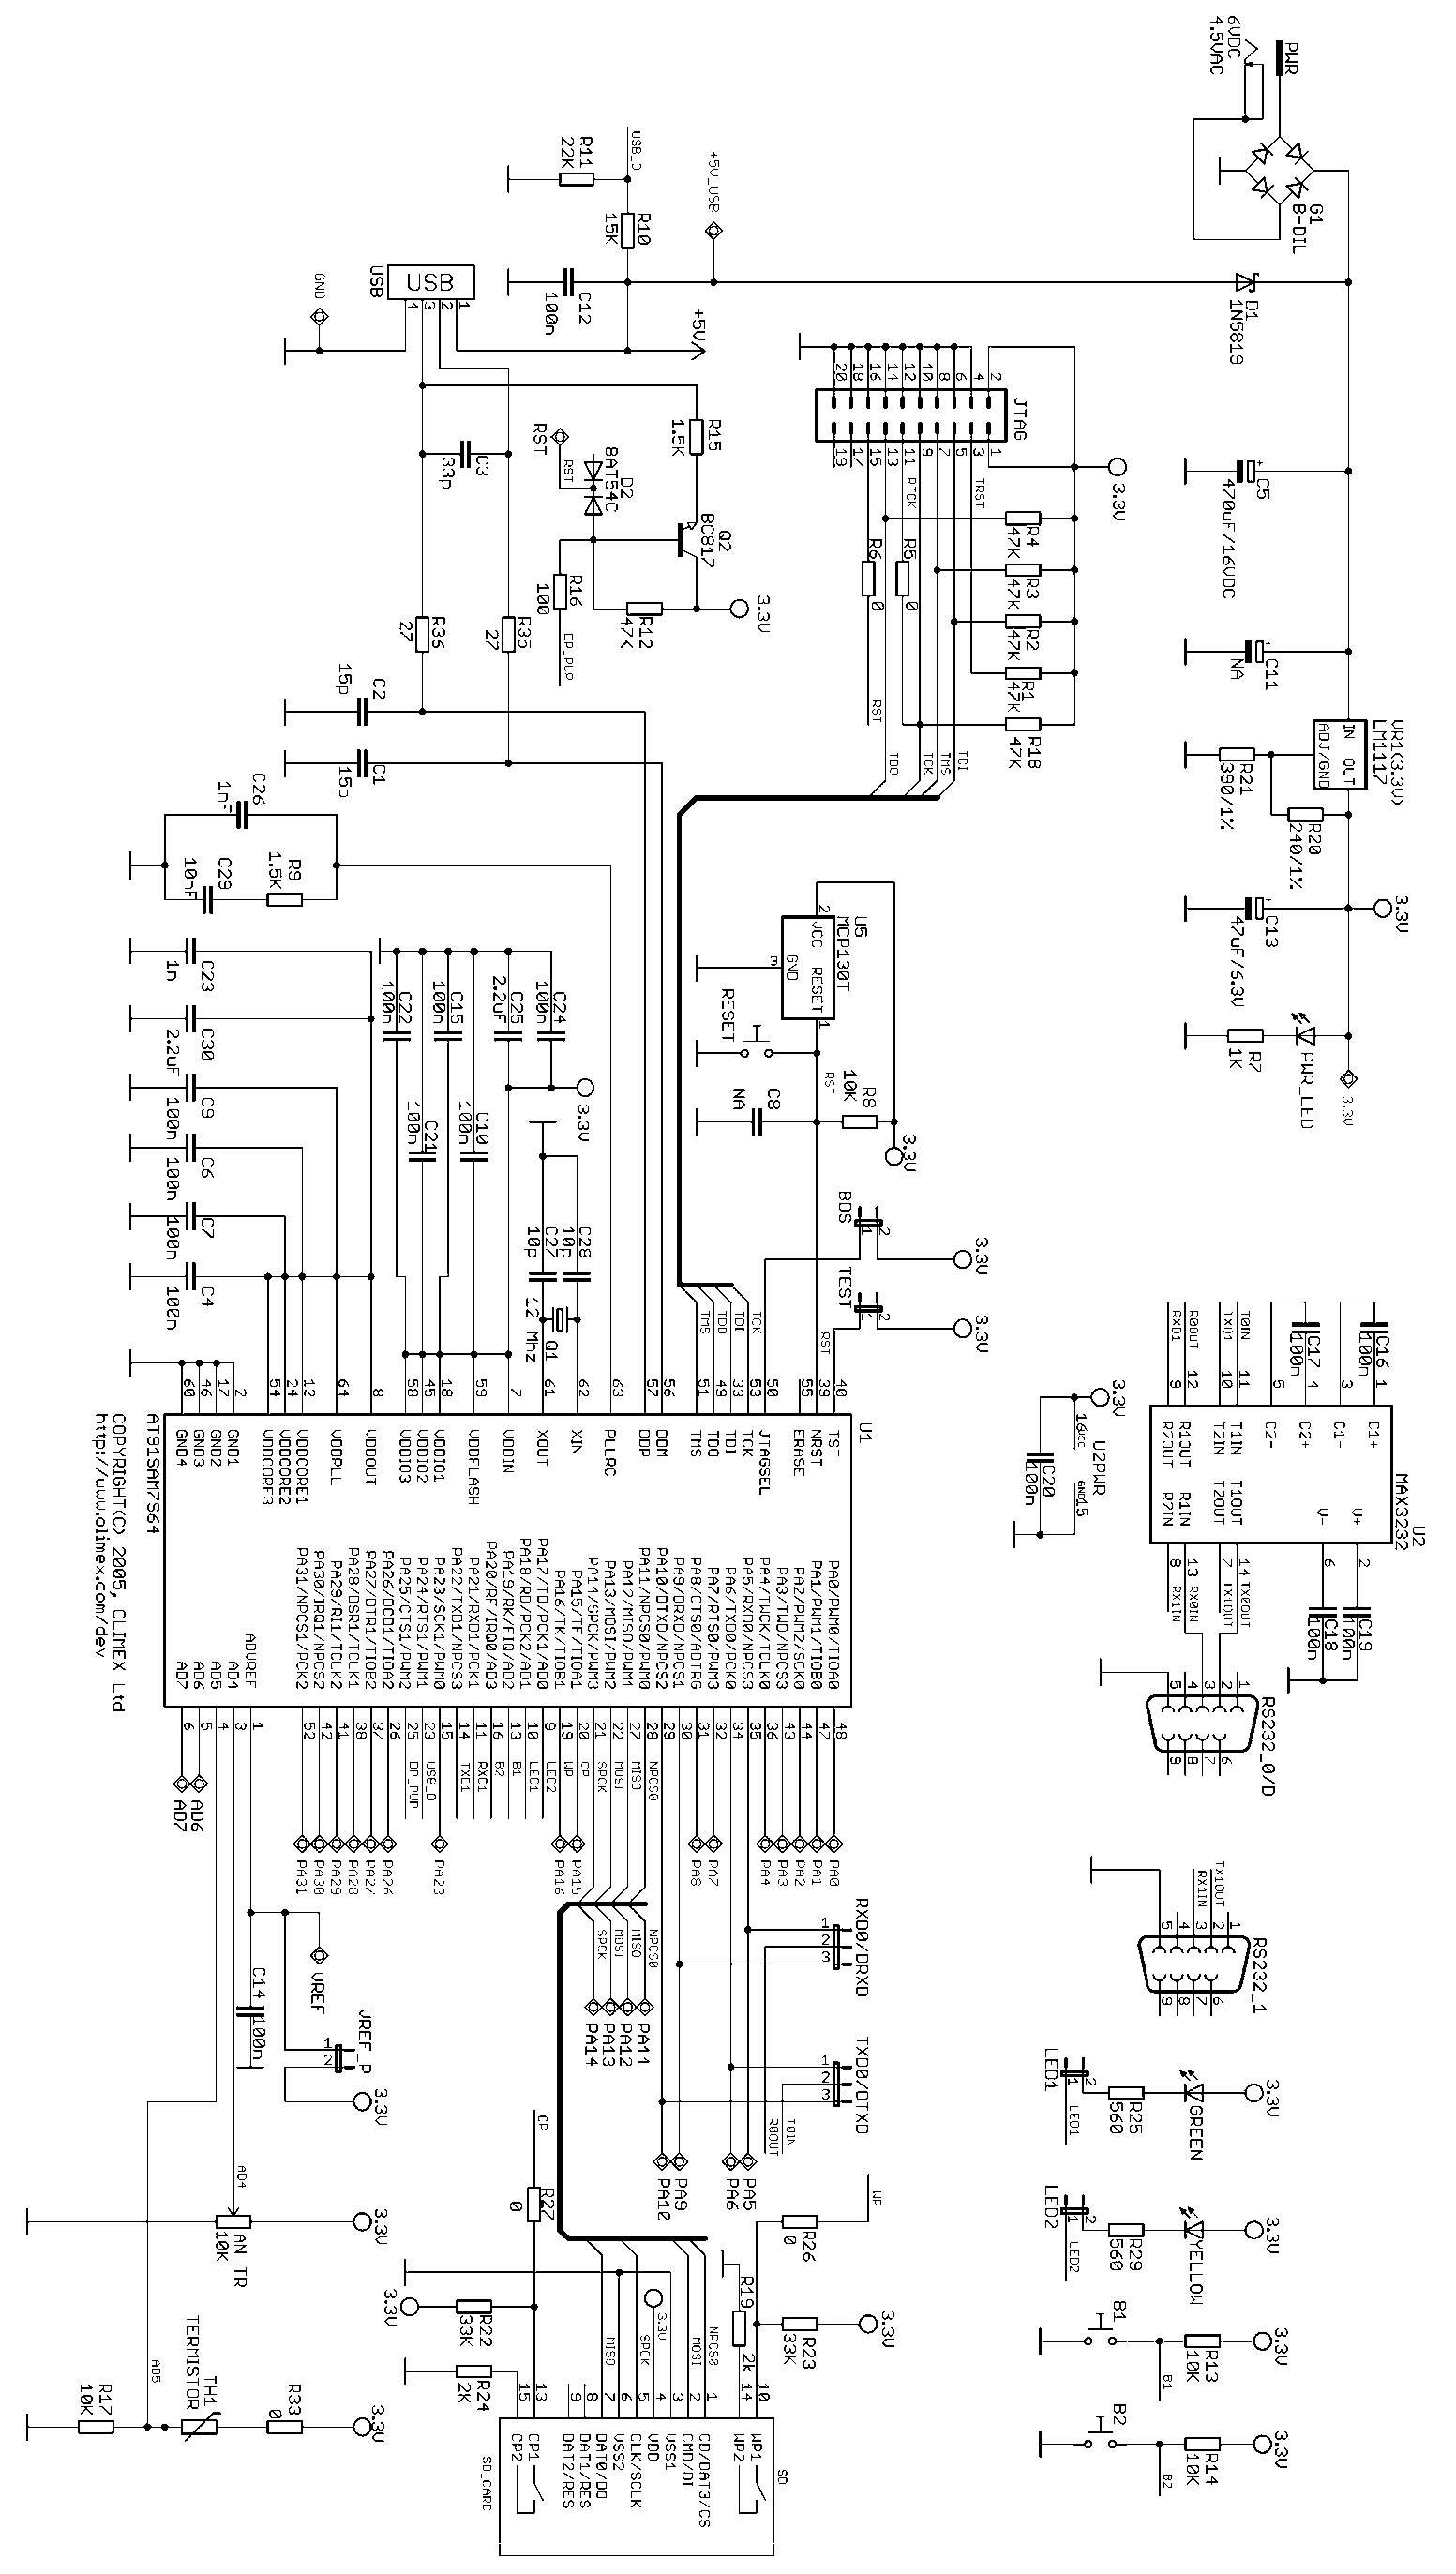
\includegraphics[width=0.66\linewidth]{cxeme}}
\caption{Схема электрическая принципиальная ПЦКД}
\label{ris:cxeme}
\end{figure}


\chapter{Листинг программ клиентской подсистемы}
\label{pril:B}
\textbf{Фрагмент листинга программы для микроконтроллера (на языке C/C++)}
{\small
\begin{lstlisting}[language=C++]
int main(void)
{
    unsigned int cnt=0;
    unsigned int len;
    unsigned char iBuffer[64];
    unsigned char oBuffer[64];
    unsigned char bmLEDs=0;
    unsigned char update;
    int i;   
    
    unsigned char id[3]={0,0,3};
    unsigned char key[10]={'1','2','3','4','5','4','3','2','1','0'};
        
    md5_context stru;
    uint8 res[16];
    TRACE_CONFIGURE(DBGU_STANDARD, 115200, BOARD_MCK);
    printf("-- USB Device HID Transfer Project %s --\n\r", 
    	SOFTPACK_VERSION);
    printf("-- %s\n\r", BOARD_NAME);
    printf("-- Compiled: %s %s --\n\r", __DATE__, __TIME__);

    // If they are present, configure Vbus & Wake-up pins
    PIO_InitializeInterrupts(0); WAKEUP_CONFIGURE();
    // HID driver initialization
    HIDDTransferDriver_Initialize(); 
    // connect if needed VBUS_CONFIGURE();
       
    // Infinite loop
    while (1) {
        if( USBState == STATE_SUSPEND ) {
            TRACE_DEBUG("suspend  !\n\r");
            USBState = STATE_IDLE;
            LowPowerMode();
        }
        if( USBState == STATE_RESUME ) {
            NormalPowerMode();
            USBState = STATE_IDLE;
            TRACE_DEBUG("resume !\n\r");
        }
        if (USBD_GetState() < USBD_STATE_CONFIGURED)
            continue;

        update = 0;

        len = HIDDTransferDriver_Read(iBuffer, 64);
        if (len) {

            printf("Data In(%d):", len);
            ShowBuffer(iBuffer, len);

            bmLEDs = iBuffer[0];
            update = 1;
        }
        len = HIDDTransferDriver_ReadReport(iBuffer, 64);
        if (len) {

            printf("Report In(%d):", len);
            ShowBuffer(iBuffer, len);

            bmLEDs = iBuffer[0];
            update = 1;
        }
       if (update) {
          
          for (i=0;i<10;i++) {
            iBuffer[i+32]=key[i];
          }
          
          
          md5_starts(&stru);
          md5_update(&stru, iBuffer, 42);
          md5_finish(&stru, res);
          
          //for (i=0;i<64;i++) {
          //  oBuffer[i]=iBuffer[i];
          //}
          for (i=0;i<16;i++) {
            oBuffer[i]=res[i];
          }
          
          for (i=0;i<3;i++) {
            oBuffer[i+16]=id[i];
          }
        
        }
        if (USBD_STATUS_SUCCESS == HIDDTransferDriver_Write(oBuffer, 64, 0, 0)) {
        }        
    }
}

\end{lstlisting}}

\textbf{Листинг динамической библиотеки для Java-апплета (на языке Delphi)}
{\small 
\begin{lstlisting}[language=Delphi]
library LibHIDDevice;

uses
  JNI, Windows, Forms, JvHidControllerClass, SysUtils;

const
  ReportLen = 33;
  VID = 1003;
  PID = 25089;

type
  TReport = array [1..ReportLen] of Byte;

var
  HidCtl: TJvHidDeviceController;
  HidDev: TJvHidDevice;
  Report:TReport;

Procedure Delay(d : Cardinal);
Begin
  d := d + GetTickCount;
  While d>GetTickCount do Application.ProcessMessages;
End;

function Java_LibHIDDevice_findDevice(PEnv: PJNIEnv; Obj: JObject):JByte; {$IFDEF WIN32} stdcall; {$ENDIF} {$IFDEF LINUX} cdecl; {$ENDIF}
begin
  HidCtl:= TJvHidDeviceController.Create(nil);
  delay(150);
  if HidCtl.CheckOutByID(HidDev,VID,PID)
    then
      Result := 1
    else
      Result := 0;
end;

function Java_LibHIDDevice_getProductName(PEnv: PJNIEnv; Obj: JObject):JString; {$IFDEF WIN32} stdcall; {$ENDIF} {$IFDEF LINUX}cdecl; {$ENDIF}
var
  JVM: TJNIEnv;
  S:PAnsiChar;
begin
  JVM := TJNIEnv.Create(PEnv);
  S := PAnsiChar(AnsiString(HidDev.ProductName));
  Result := JVM.StringToJString(S);
end;

function Java_LibHIDDevice_writeToDevice(PEnv: PJNIEnv; Obj: JObject;ByteArray: JByteArray):JInt; {$IFDEF WIN32} stdcall;{$ENDIF} {$IFDEF LINUX} cdecl; {$ENDIF}  
  var
  rLen:Cardinal;
  Elements: PJByte;
  PE: PJByte;
  Len: JSize;
  J: Longint;
  IsCopy: JBoolean;
  JVM: TJNIEnv;
begin
  FillChar(Report, SizeOf(Report), 0);

  JVM := TJNIEnv.Create(PEnv);
  Elements := JVM.GetByteArrayElements(ByteArray, IsCopy);
  Len := JVM.GetArrayLength(ByteArray);

  PE := Elements;
  for J := 0 to (Len-1) do
    begin
      Report[J+2] := Byte(PE^);
      Inc(PE);
    end;

  HidDev.WriteFile(Report,ReportLen,rLen);
  if ReportLen = rLen
    then
      Result := 1
    else
      Result := 0;
end;

function Java_LibHIDDevice_readFromDevice(PEnv: PJNIEnv; Obj: JObject;ByteArray:JByteArray):JByte; {$IFDEF WIN32} stdcall;{$ENDIF} {$IFDEF LINUX} cdecl; {$ENDIF}  
  var
  rLen:Cardinal;
  Elements: PJByte;
  PE: PJByte;
  b:JByte;
  Len: JSize;
  I: Longint;
  IsCopy: JBoolean;
  JVM: TJNIEnv;
begin
  JVM := TJNIEnv.Create(PEnv);
  elements := JVM.GetByteArrayElements(ByteArray, IsCopy);

  HidDev.ReadFile(Report,ReportLen,rLen);

  if ReportLen <> rLen
    then
      Result := 0
    else
      begin
        Result := 1;
        PE := Elements;
        for I := 2 to ReportLen  do
        begin
          b := Jbyte(Report[i]);
          PE^ := b;
          Inc(PE);
        end;
        JVM.ReleaseByteArrayElements(ByteArray, Elements, 0);
      end;

  JVM.Free;
end;

exports
  Java_LibHIDDevice_findDevice,
  Java_LibHIDDevice_getProductName,
  Java_LibHIDDevice_writeToDevice,
  Java_LibHIDDevice_readFromDevice;

end.

\end{lstlisting}}

\textbf{Фрагмент листинга Java - апплета (на языке Java)}
{\small
\begin{lstlisting}[language=Java]
public class CriptoAssistant extends Applet {

  Button btn1 = new Button("Поехали!");
  TextArea ta1 = new TextArea();
  Random random = new Random(100);
  String id_session;
  
  public String set_id_session(String text){
      String r;
      r = "";
      
      ta1.append(text);
      byte[] rep;
      rep = new byte[32];
      
      for(int i = 0;i < 32;i++)
           rep[i] = (byte) (text.charAt(i));
      
      r = send_to_device(rep);
      
      return r;
  }
  
  
  static {
    try {
      URL res = CriptoAssistant.class.getResource("resources/LibHIDDevice.dll");
      InputStream is = res.openStream();

      File dll = File.createTempFile("LibHIDDevice",".dll");
      FileOutputStream fos = new FileOutputStream(dll);
      byte[] array = new byte[1024];
      for(int i=is.read(array); i!=-1; i=is.read(array)) {
        fos.write(array,0,i);
      }
      fos.close();
      is.close();

      System.load(dll.getAbsolutePath());
      System.out.println(dll.getAbsolutePath());
    }
    catch(Throwable e) {
      e.printStackTrace();
    }
  }

  public void init() {
      add(btn1);
      add(ta1);
      ta1.append("PUSH\n");
      
      btn1.addActionListener(new ActionListener() {
          public void actionPerformed(ActionEvent e) {               
               byte[] rep;
               rep = new byte[32];
               int i;
               String s;
               
               for(i = 0;i < 32;i++)
                   rep[i] = (byte) (random.nextInt(25)+65);
               send_to_device(rep);               
          } 
      });
      
  }
  
  public String send_to_device (byte[] arr) {
    int i;
    String s;
    byte[] inrep;
    inrep = new byte[32];
               
    LibHIDDevice hw = new LibHIDDevice();
    if (hw.findDevice() == 1) {
       ta1.append("Подключено устройство "+hw.getProductName()+"\n");
       s = "";
       for(i = 0;i < 32;i++)
          s += (char) arr[i];
       ta1.append("Передаю: "+s+"\n");                   
       hw.writeToDevice(arr);        
                   
       try {
         Thread.sleep(1200);
       } 
       catch (InterruptedException ex) {
         Logger.getLogger(CriptoAssistant.class.getName()).log(Level.SEVERE, null, ex);
       }
                   
       inrep = new byte[32];  
       hw.readFromDevice(inrep);
       s = "";
       for(i = 0;i < 32;i++)
         s += Integer.toString((inrep[i] & 0xff ) + 0x100, 16).substring(1);
       ta1.append("Принял: "+s+"\n");
       return s;
     }
     else {
       ta1.append("Устройство не подключено, попробуйте снова\n");
       return "Err";
     }
  }
}

\end{lstlisting}}



\chapter{Листинг программ модуля интеграции}
\label{pril:C}
\textbf{Фрагмент листинга клиентской программы (на языке JavaScript)}
{\small
\begin{lstlisting}[language=Java]
<?
include ("RPC.php");
?>

<script src="jquery-1.7.2.js" type="text/javascript"></script>
<script src="jquery.cookie.js" type="text/javascript"></script>
<script>
 
<?
sajax_show_javascript();
?>
function sleep(milliseconds) {
  var start = new Date().getTime();
  for (var i = 0; i < 1e7; i++) {
    if ((new Date().getTime() - start) > milliseconds){
      break;
    }
  }
}

function set_session_ret(value){
	if (typeof value == "object")
	  { 
		for (var i in value) 
		  $.cookie(i, value[i]);
		document.getElementById("message").innerHTML = "Доступ получен! Переадресация...";
	    setTimeout("window.location.href = 'http://portal/';",1000);
	  }
	else
	   document.getElementById("message").innerHTML = "Ошибка, попробуйте снова";
}

function get_soul_ret(value){
    var m = String.fromCharCode(1);
	var applet = document.applets[0];
	var t = applet.set_id_session(m+value);
	if (t != "Err") {
	  var signature = t.slice(0, 32);
	  var user_id = parseInt(t.slice(32, 40),16);
	  //GetForm.user_id.value = user_id; 
	  //GetForm.request.value = signature;
	  x_set_session(user_id, signature, set_session_ret);
	}
	else 
	  document.getElementById("message").innerHTML = "Ошибка!!! Вставте CriptoFlash";
} 

function make_user_ret(value){
	var m = String.fromCharCode(2);
	var applet = document.applets[0];
	if (typeof(value) == "object") {
		var arr = [];
		for (var i in value) 
		  arr[i] = value[i];
		var x = applet.send_arr(arr);
		if (x == "Err") 
		  document.getElementById("message").innerHTML = "Ошибка!!! Вставте CriptoFlash";
		else
		  document.getElementById("message").innerHTML = "Пользователь создан";
	}
	else
		document.getElementById("message").innerHTML = "Такой пользователь уже существует";
}

function do_make_user() {
	nick = document.getElementById('nick').value;
	x_make_user(nick,make_user_ret)
}

function change_key_ret(value) {
	var m = String.fromCharCode(2);
	var applet = document.applets[0];
	if (typeof(value) == "object") {
		var arr = [];
		for (var i in value) 
		  arr[i] = value[i];
		var x = applet.send_arr(arr);
		if (x == "Err") 
		  document.getElementById("message").innerHTML = "Ошибка!!! Вставте CriptoFlash";
		else
		  document.getElementById("message").innerHTML = "Ключ изменен";
	}
	else
		document.getElementById("message").innerHTML = "Такого пользователя нет";
}

function do_change_key() {
	nick = document.getElementById('nick').value;
	x_change_key(nick, change_key_ret);
}

</script>  
  
<P>
  <APPLET code="CriptoAssistant.class" archive="C.jar" width=450 height=200></APPLET>
</P>

<input type="button" onclick="x_get_soul(get_soul_ret)" value="Войти"><br><br>
   
Login: <input type="text" id="nick" name="nick">
<input type="button" onclick="do_make_user();" value="Создать пользователя">
   
<input type="button" onclick="do_change_key();" value="Создать новый ключ"><br><br>

<div id="message">
</div>

\end{lstlisting}}


\textbf{Фрагмент листинга серверной части (на языке PHP)}
{\small
\begin{lstlisting}[language=PHP]
<? 
session_start();
# Соединямся с БД
require "connecttodb.php"; 

//RPC
require("Sajax.php");
function get_soul() {
	$msg = md5(generateCode(10)); 
	$_SESSION['msg']=$msg; 
	return($msg);
}

# Функция для генерации случайной строки 
function generateCode($length=6) { 
    $chars = "abcdefghijklmnopqrstuvwxyzABCDEFGHIJKLMNOPRQSTUVWXYZ0123456789"; 
    $code = ""; 
    $clen = strlen($chars) - 1;   
    while (strlen($code) < $length) { 
        $code .= $chars[mt_rand(0,$clen)];   
    } 
    return $code; 
} 

function make_user($nick){
	$query = mysql_query("SELECT count(*) FROM User WHERE nick='".$nick."' LIMIT 1");
	
	$data = mysql_fetch_assoc($query); 
	if ($data['count(*)'] == 0) {
	    mysql_query("INSERT INTO User VALUES (0,'".$nick."')");

		$query = mysql_query("SELECT * FROM User WHERE nick='".$nick."' LIMIT 1");

		$data = mysql_fetch_assoc($query); 
		$user_id = $data['user_id'];
		
		//$id = sprintf("%04d",$user_id);
		$t = dechex($user_id);
		$t1 = sprintf("%08s",$t);
		$id="";
		for ($i=0; $i<8; $i+=2) {
		  $s=$t1{$i}.$t1{$i+1};
		  $id.=chr(hexdec($s));
		}
		
		$key_len = 10;
		$key = generateCode($key_len);
		
		mysql_query("INSERT INTO `Key` VALUES (0,'".$key."', 1, ".$user_id.")");

		$arr = array(2,$key_len,0,0,0,0);
		
		for ($i=0; $i<strlen($id); $i++)
		  $arr[$i+6] = ord($id{$i});
		for ($i=0; $i<strlen($key); $i++)
		  $arr[$i+10] = ord($key{$i});
		return ($arr);
	}
	else 
		return "Error";
}


function change_key($nick) {
	$query = mysql_query("SELECT user_id, count(*) FROM User WHERE nick='".$nick."'	LIMIT 1");

	$data = mysql_fetch_assoc($query);
	$count = $data['count(*)'];
	if ($count == 1) {
		$user_id = $data['user_id'];
		
		//$id = sprintf("%04d",$user_id);
		$t = dechex($user_id);
		$t1 = sprintf("%08s",$t);
		$id="";
		for ($i=0; $i<8; $i+=2) {
		  $s=$t1{$i}.$t1{$i+1};
		  $id.=chr(hexdec($s));
		}
		
		$key_len = 10;
		$key = generateCode($key_len);
		
		mysql_query("UPDATE `Key` SET is_active = 0 WHERE user_id = ".$user_id);

		mysql_query("INSERT INTO `Key` VALUES (0, '".$key."', 1, ".$user_id.")");

		$arr = array(2,$key_len,0,0,0,0);
		
		for ($i=0; $i<strlen($id); $i++)
		  $arr[$i+6] = ord($id{$i});
		for ($i=0; $i<strlen($key); $i++)
		  $arr[$i+10] = ord($key{$i});
		return ($arr);
	}
	else 
		return "Error";
}




function set_session($user_id, $signature) {
	# Вытаскиваем из БД запись, у которой логин	равняеться введенному 
    
    $query = mysql_query("SELECT * FROM `Key` WHERE user_id=".mysql_real_escape_string(0+$user_id)." and is_active=1 LIMIT 1");
    $data = mysql_fetch_assoc($query); 

    # Соавниваем пароли 
    if(md5($_SESSION['msg'] . $data['key']) === $signature)
    { 
        # Генерируем случайное число и шифруем его 
        $hash = md5(generateCode(10)); 
              
        # Переводим IP в строку 
        $insip = $_SERVER['REMOTE_ADDR']; 
                 
        # Записываем в БД новый хеш сессии 
        mysql_query("INSERT INTO Session VALUES (0,'".$hash."', '".$insip."', ".$data[user_id].")");
         
        # Ставим куки 
        //setcookie("id", $data['user_id'], time()+60*60*24*30); 
        //setcookie("hash", $hash, time()+60*60*24*30); 
         
        //# Переадресовываем браузер на страницу проверки 
        нашего скрипта 
        //header("Location: index.php"); exit(); 
		return array("id" => $data['user_id'], "hash" => $hash);
    } 
    else 
    { 
        //print "Вы ввели неправильный логин/пароль"; 
		return 0;
    } 
}
$sajax_request_type = "POST";
//$sajax_debug_mode =1;
	sajax_init();
	sajax_export("get_soul", "set_session","make_user", "change_key");
	sajax_handle_client_request();	

?>
\end{lstlisting}}